%!TEX root = ../thesis.tex

\section{Data Generation}
% Give quick intro into what kind of data is needed for a DL approach.
In deep learning, one basically tries to fit a mathematical model, the neural
network, to a data set consisting of measurements. This process is called
\textit{learning}.
Those measurements might be data from a physical experiment, time series from
the stock market, health information collected for mice or virtually any
other source of data.

In most cases, the data is split into three sets. The first subset is used to
train the neural network and is called \textit{training set}. The second subset 
is used to validate the learning progress and is called \textit{validation set}.
This process of learning and validating is repeated until we think the trained
NN can make good predictions. In a last step we use the trained NN to make an
unbiased prediction on the third subset, called \textit{test set}.

In the case of GW we only have a very limited data set of measurements. We can't
make an experiment to easily generate more measurements, we can only try to 
detect the ones which occure naturally. This rises the problem of needing to 
know how a gravitational wave looks like to be able to measure it. We solve this
by simulating GW waveforms and injecting it into Gaussian noise.

\subsection{Training and Validation Set}
% Parameters for signal
To generate the training and validation set, we first generate $100'000$ GW signal
waveforms sampled at 2048 Hz. The two masses $m_1$ and $m_2$ are drawn uniformly
between $10 \textup{M}_\odot$
and $50 \textup{M}_\odot$ whereas $m_1 < m_2$. The \textit{coalescence phase},
\textit{inclination} and \textit{polarization angle} are drawn uniformly between
$0$ and $2 \pi$. Furthermore we use
pyCBC's \hlc{sky\_location.UniformSky()} to compute the \textit{declination} and
\textit{right ascention}. We also use a \textit{low frequency cutoff} of 18 Hz.
We use the \hlc{SEOBNRv4\_opt} approximant to generate the waveforms. Those
choices are motivated by \cite{PhysRevD.105.043002} and \cite{MLGWSC1}. 
Note that here, the sky 
location as well as the inclination and polarization are set from the start.

The NN which will be used in this thesis \cite{PhysRevD.105.043002} assumes
the training and validation set to cointain 1 second long samples yet the 
generated waveforms will end up having 
a duration of several seconds. We solve this problem by choosing a 1.25 second
window around the merger. This leads to the merger being always placed in
the middle of the window. Since a NN is likely to learn such positional
information, we vary the placement of the window randomly by 0.2
seconds. This way, the mergers placement won't be fixed, adding stability to our
NN. \autoref{fig:2_cutting_windows} shows three such choices for a
window containing the merger whereas green is the maxiaml variation towards the
left, red is without variation and yellow is the maximal variation towards the
right. Limiting the variation by 0.2 seconds is an arbritary choice.

\begin{figure}[t]
  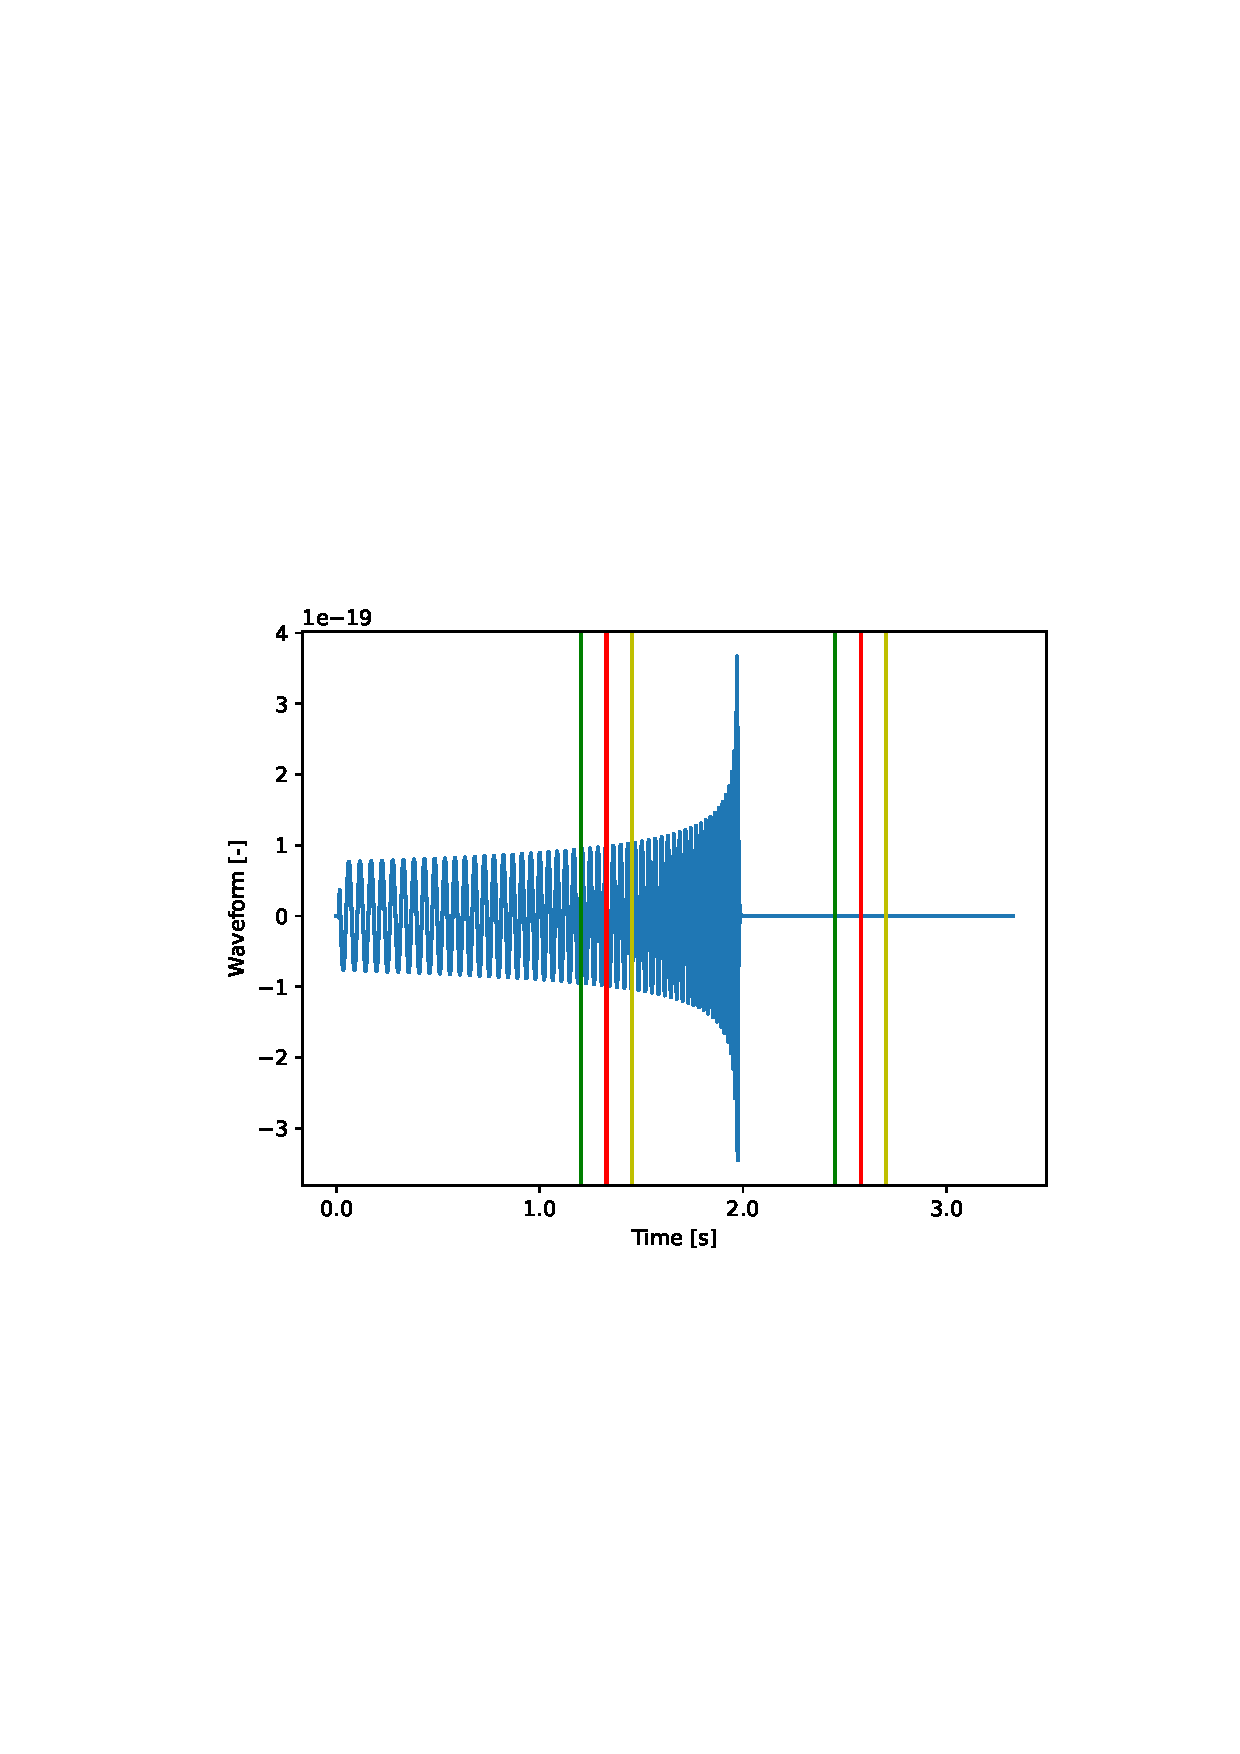
\includegraphics[width=\textwidth]{img/2_data_generation/chapter2_cutting_window.png}
  \caption{Cutting windows varied by \textcolor{green!40!black}{-0.2s},
    \textcolor{red}{0.0s} and \textcolor{yellow!60!black}{+0.2s}}
  \label{fig:2_cutting_windows}
  \centering
\end{figure}

% Parameters for noise
Next we generate $200'000$ pure Gaussian noise samples sampled at 2048 Hz with
a duration of 1.25 seconds.
The noise is generated using pyCBC's implementation of
\hlc{aLIGOZeroDetHighPower} PSD with a low frequency cutoff of $18$ Hz
\cite{PhysRevD.105.043002} \cite{MLGWSC1}.

% Generating samples
At last we need to generate the actual samples used to train and validate the NN
. This is done by injection all $100'000$ signal waveforms into $100'000$ of the
$200'000$ noise samples. We end up with $100'000$ pure Gaussian noise samples
and $100'000$ samples of signals injected into Gaussian noise.

From \cite{PhysRevD.105.043002} we see that the best training is done on samples
with SNR
of 8. This is because DL algorithms can generalize low SNR signals to high SNR
ones while the converse is not true. \cite{PhysRevD.105.043002} 
Because of this, we rescale
the signals to have an SNR of 8 before injecting them into the Gaussian noise.

In a last step, all $200'000$ samples are whitened, leading to corrupted edges.
Removing the corrupted edges reduces the duration of each sample from
1.25 second to 1 second. This corruption of the edges happens because the
algorithm implementing whitening
assumes periodicity of the data while the data isn't periodic. This assumption
stems from the fact that analtically, whitening assumes an infinite time series.
\footnote{Discussed with Ondřej Zelenka on 10.12.2021 in a private Slack
  conversation.} 

We end up with $200'000$ samples of 1 second whereas half of it contains a signal
and the other half doesn't. We say they have the labels \textit{pure noise} and 
\textit{noise+signal}. Those $200'000$ samples will then be split into
training and validation set using a 80/20 split. Before the split, the samples
are shuffled uniformly leading to a similar ratio between
pure noise and noise+signal samples in both sets. There is no mechanism in place
to enforce an equal ratio.

\subsubsection{Implementation}
Generating the above described data is implemented in the file \\
\hlc{generate\_training\_data.py} found in the \hlc{scripts} folder. It utilizes
the classes \hlc{SignalSpace}, \hlc{SignalGenerator}, \hlc{NoiseSpace},
\hlc{NoiseGenerator}, \hlc{SampleSpace} and \hlc{SampleGenerator}. We can divide
all those classes into two categories: \hlc{Spaces} and \hlc{Generators}. The
\hlc{Spaces} provide the parameters used to generate noise, signals or samples
and the \hlc{Generators} takes one set of parameters to generate the noise,
signal or sample using its \hlc{generate(params)} method.

The data generation is a computationally expensive task. If implemented
sequentially\footnote{Sequentially means one task is executed after the other,
basically running it on one core.} it can take
up to a day or even longer, depending on the approximant used and the
amount of data generated. To drastically reduce the time needed for data
generation, I parallelized\footnote{Parallelization is the task of implementing
an algorithm in a way such that it can run on several cores simultaneously.
Reducing its execution time.} it using a \textit{master-slave} approach
implemented using MPI\footnote{resp. the Python wrapper mpi4py}. In
this approach one core, the master, distributes a batch of work and the slaves
execute this batch of work. Once a slave is done it asks the master for more
work.

This approach was chosen because the computational work differs from
sample to sample which means that if we were to distribute all the work in the
beginning, we wouldn't utilize the full power of all cores. Furthermore this
approach also made it easy to ensure that
all work is generated from the same \hlc{Space} (i.e. distribution) which is
important because we use several random number generators. This choice
also gives a lot of flexibilty, which is important when working with DL since
it allows you to easier iterate over ideas.

The data generation was run on ETH's Euler cluster which acts as a distributed
system and is the reason we chose MPI instead of e.g. openMP to parallelize the
data generation.

\subsection{Test Set}
The test set consists of 1 month of data. Note that this is different to the
training and validation set since those used samples of a duration of 1 second
while here we basically have one sample with a duration of 1 month. This is
needed to address the issues describes in \cite{PhysRevD.100.063015}.

The test set is being generated by utilizing the \hlc{generate\_data.py} script
from \cite{MLGWSC1}. Note that \cite{MLGWSC1} provides the possibility of
generating test data on 4 complexity level. The first one being Guassian noise
and simulated signals while the last one is basically real LIGO-Virgo data.

The reason it was used is because it gives the possibility to easily test the
trained NN on more complex test data. Note that in this thesis, only the simplest
test set was used.

This script will generate two datasets. One fore the so called
\textit{foreground data} and another for the so called \textit{background data}.
The difference is that the background data only contains the pure noise
while the foreground has signals injected into it as described in the
\textit{injections} file. Having both files allows us to conpate false positives
with true positives which in turn is needed to compute metrics.

Note that a LIGO observation run is split into time segments which indicate
the time intervals in which the measured data was of sufficient quality. While
the injections file contains injections for the whole duration of an
obervation run i.e. ignores the segments, the \hlc{generate\_data.py} script
only chooses injections which are at a time contained in one of the segments. In
the generated HDF file, each such segment is stored in its own dataset.

Since our training data consists of whitened samples, we also have to whiten the
test data. This is done by whitening each segment at once, again resulting in a
data loss of $0.25$s for each segment. In total, we lose $32.5$ seconds after
whitening the whole month of data. Whitening here is done by the \hlc{whiten.py}
script provided in \cite{MLGWSC1}. This script again utilizes the \hlc{whiten}
function of pyCBC but also allows you to provide the noise PSD explicitly. In
case it isn't provided explicitly, it tries to estimate it from the given strain
. Having these features is especially important when working with the more
complex data sets.

